\chapter{CNNs Models}
\label{chp:mds}
There are two CNNs proposed to accomplish the dynamic hand posture recognition task.
A straight forward method of template matching is employed at first, followed by a network of multi-layer perceptrons (MLP) trained to improve the recognition performance.


\begin{figure}
\centering
	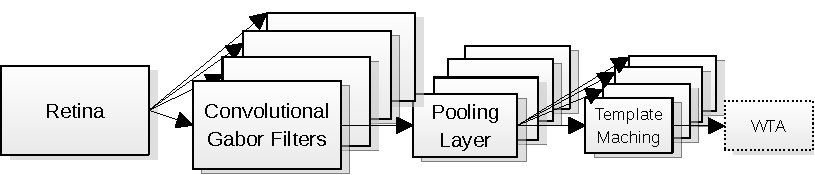
\includegraphics[width=0.8\textwidth]{pics/model1.pdf}
	\caption{Model 1. 
	The retina input is convolved with Gabor filters in the second layer, and then shrinks the sizes in the pooling layer.
	The templates are considered as convolution kernels in the last layer.
	The WTA circuit can be used as an option to show the template matching result more clearly.
	}
	\label{fig:model1}
\end{figure}
%\subsubsection{Model 1. Template Matching}

Model 1: Template Matching. Shown in Figure~\ref{fig:model1} the first layer is the retina input, followed by the convolutional layer, where the kernels are Gabor filters responding to edges of four orientations.
The third layer is the pooling layer where the size of the populations shrinks. 
This down-sampling enables robust classification due to its tolerance to variations in the precise shape of the input. 
The fourth layer is another convolution layer where the output from the pooling layer is convolved with the templates.
The optional layer of Winner-Take-All (WTA) neurons enables a clearer classification result due to the inhibition between the neurons.
In the Matlab simulation, the retina input spikes are buffered into 30~ms frames, and the neurons are simple linear perceptrons.
The templates are chosen by sampling the output of the pooling layer when given some reference stimulus, see Figure~\ref{fig:template}.

\begin{figure}
\centering
	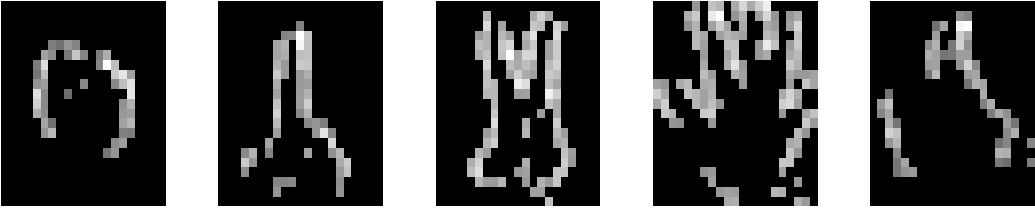
\includegraphics[width=0.8\textwidth]{pics/gesture.pdf}
	\caption{Templates of the five postures: `Fist',`Index Finger', `Victory Sign', `Full Hand' and `Thumb up'.}
	\label{fig:template}
\end{figure}

The Gabor filter is well-known as a linear filter for edge detection in image processing. 
A Gabor filter is a 2D convolution of a Gaussian kernel function and a sinusoidal plane wave; see Equation~\ref{equ:gabor}. 
\begin{equation}
\begin{array}{l}
\mathrm{Real Parts} = \exp \left(\frac{-x^{'2}+y^{'2}}{2\sigma ^{2}}\right)\cos \left(2\pi\frac{{x}'}{\lambda }\right)
\\
\\
\mathrm{Imaginary Parts} = \exp \left(\frac{-x^{'2}+y^{'2}}{2\sigma ^{2}}\right)\sin \left(2\pi\frac{{x}'}{\lambda }\right)
\\
\\
\mathrm{where:}
\\
\\
{x}'=x\cos (\theta ) + y\sin (\theta)
\\
\\
{y}'=-x\sin (\theta ) + y\cos (\theta)
\end{array}
\label{equ:gabor}
\end{equation}
$\theta$ represents the orientation of the filter, $\lambda$ is the wavelength of the sine wave, and $\sigma$ is the standard deviation of the Gaussian envelope. 
The frequency and orientation features are similar to the responses of V1 neurons in the human visual system. 
Only the real parts of the Gabor filters (see Figure~\ref{fig:gabor}) are used as the convolutional kernels to configure the weights between the input layer and the Gabor filter layer.

\begin{figure}
\centering
	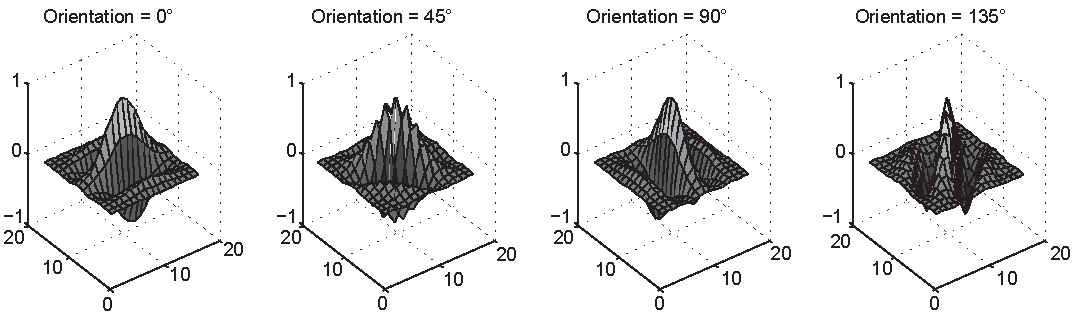
\includegraphics[width=0.8\textwidth]{pics/gabor.pdf}
	\caption{Real parts of the Gabor filters orienting four directions.}
	\label{fig:gabor}
\end{figure}

%The templates (see Figure~\ref{fig:template}) are manually selected from the output of the pooling layer in the framed Matlab simulation. 
The output score of a convolution is determined by the matching degree between the input and the kernel.
Regarding the template matching layer, each neuron in a population responds to how closely its receptive field matches the specific template.
The position of moving gesture is also naturally encoded in the address of template matching neuron.
Thus, there are five populations of template matching neurons, one for each hand posture listed.

%\subsubsection{Model 2. Trained MLP}
Model 2: Trained MLP. 
Inspired by the research of Lecun~\cite{lecun1998gradient}, we designed a combined network model with MLP and CNN (Figure~\ref{fig:model2}). 
The first three layers are exactly the same as the previous model.
The training images for the 3-layered MLP are of same size and the posture is centred in the images.
Therefore, a tracking layer plays an important role to find the most active region and forward the centred image to the next layer.

\begin{figure}
\centering
	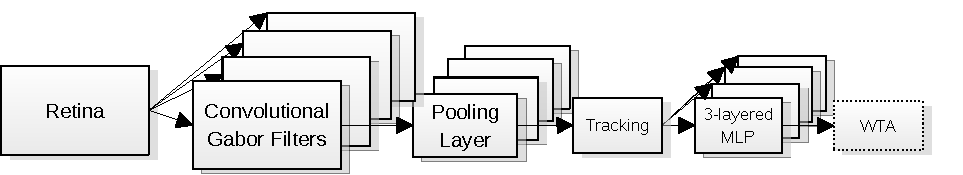
\includegraphics[width=0.8\textwidth]{pics/model2.pdf}
	\caption{Model 2. 
	The retina input convolves with Gabor filters in the second layer, and then shrinks the sizes in the pooling layer.
	The following tracking layer finds the most active area of some fixed size, moves the posture to the centre and pushes the image to the trained MLP.
	The winner-take-all (WTA) layer can be used as an option to show the template matching result more clearly.}
	\label{fig:model2}
\end{figure}

%Since the size of the input image of the MLP training is fixed and the position is centered, tracking plays a very important role to spot the valid region. 
%Tracking is naturally embedded in the pooling layer of the convolutional network, for the active neurons directly point out the lively receptive field. 

\subsection{Experimental Set-up}
\label{sec:tat}
In order to evaluate the cost and performance trade-offs in optimizing the number of neural components, both the convolutional models described above are tested at different scales. 
Five videos of every posture are captured from the silicon retina in AER format, all of similar size and moving clock-wise in front of the retina. 
The videos are cut into frames (30~ms per frame) and presented to the convolutional networks. 
The configurations of the networks are listed in Table~\ref{tbl:nns}.
The integration layer is not necessary in a convolutional network, but is used here to decrease the number of synaptic connections.

\begin{table}
\caption{Sizes of the convolutional neural networks.}
	\begin{subtable}{0.6\textwidth}
		
		\centering
		\caption{Model 1: Template matching}
		\begin{tabular}{p{0.26\textwidth}|p{0.3\textwidth}<{\centering}|p{0.26\textwidth}<{\centering}|p{0.26\textwidth}<{\centering}|p{0.26\textwidth}<{\centering}}
		%Line 1
		\Xhline{1.2pt}
		    & \multicolumn{2}{c|}{\tabincell{c}{\textbf{Full Resolution } \\\textbf{128 $\times$ 128}}}  
		    & \multicolumn{2}{c}{\tabincell{c}{\textbf{Sub-sampled Resolution} \\\textbf{32 $\times$ 32}}}
		    \\ \cline{2-5}
		%Line 2
			& \tabincell{c}{Population \\ Size}
			& \tabincell{c}{Connections \\ per Neuron}
			& \tabincell{c}{Population \\ Size}
			& \tabincell{c}{Connections \\ per Neuron}
			\\ \Xhline{1.2pt}
		%Line 3
		\tabincell{l}{\textbf{Retinal} \\\textbf{Input}}
			& 128 $\times$ 128	& 1	& 32 $\times$ 32	& 4 $\times$ 4
			\\ \hline
		%Line 4
		\tabincell{l}{\textbf{Gabor} \\\textbf{Filter}}
			& 112$\times$112$\times$4	& 17 $\times$ 17	& 28$\times$28$\times$4	& 5 $\times$ 5
			\\ \hline
		%Line 5
		\tabincell{l}{\textbf{Pooling} \\\textbf{Layer}}
			& 36$\times$36$\times$4	& 5 $\times$ 5	& null	& null
			\\ \hline
		%Line 6
		\tabincell{l}{\textcolor[rgb]{0.55,0.55,0.55}{\textbf{Integration}} \\ \textcolor[rgb]{0.55,0.55,0.55}{\textbf{Layer}}}
			& 36 $\times$ 36	& 4	& 28 $\times$ 28	& 4
			\\ \hline
		%Line 7
		\tabincell{l}{\textbf{Template} \\\textbf{Matching}}
			& 16$\times$16$\times$5	& 21 $\times$ 21	& 14$\times$14$\times$5	& 15 $\times$ 15
			\\ \Xhline{1.2 pt}
		%Line 8
		\textbf{Total}
			& $74,320$	& $15,216,512$	& $5,925$	& $318,420$
			\\ \Xhline{1.2 pt}
		\end{tabular}
		\label{tbl:m1}
	\end{subtable}
	\par\bigskip
	\begin{subtable}{0.6\textwidth}
		
		\centering
		\caption{Model 2: Trained MLP}
		\begin{tabular}{p{0.26\textwidth}|p{0.3\textwidth}<{\centering}|p{0.26\textwidth}<{\centering}|p{0.26\textwidth}<{\centering}|p{0.26\textwidth}<{\centering}}
		%Line 1
		\Xhline{1.2pt}
		    & \multicolumn{2}{c|}{\tabincell{c}{\textbf{Full Resolution} \\\textbf{128 $\times$ 128}}}  
		    & \multicolumn{2}{c}{\tabincell{c}{\textbf{Sub-sampled Resolution} \\\textbf{32 $\times$ 32}}}
		    \\ \cline{2-5}
		%Line 2
			& \tabincell{c}{Population \\ Size}
			& \tabincell{c}{Connections \\ per Neuron}
			& \tabincell{c}{Population \\ Size}
			& \tabincell{c}{Connections \\ per Neuron}
			\\ \Xhline{1.2pt}
		%Line 3
		\tabincell{l}{\textbf{Tracked} \\\textbf{Input}}
			& 21 $\times$ 21	& null	& 15 $\times$ 15	& null
			\\ \hline
		%Line 4
		\tabincell{l}{\textbf{Hidden} \\\textbf{Layer}}
			& 10	& 21$\times$21$\times$10	& 10	& 15$\times$15$\times$10
			\\ \hline
		%Line 5
		\tabincell{l}{\textbf{Recognition} \\\textbf{Layer}}
			& 5	& 5$\times$10	& 5	& 5$\times$10
			\\ \Xhline{1.2pt}
		%Line 6
		\textbf{Total}
			& $456$	& $4,460$	& $240$	& $2,300$
			\\ \Xhline{1.2 pt}
		\end{tabular}
		\label{tbl:m2}
	\end{subtable}
	\label{tbl:nns}
\end{table}

\subsection{Experimental Results}
\label{sec:exp}

\begin{figure}
\centering
	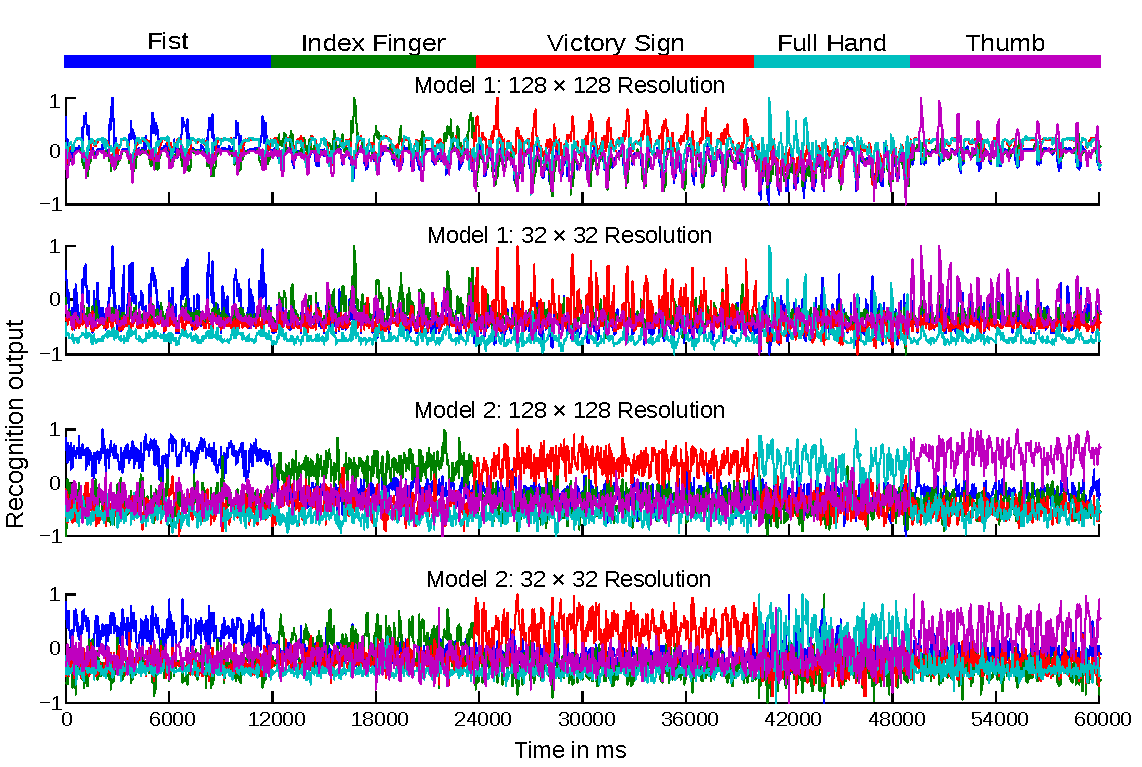
\includegraphics[width=0.8\textwidth]{pics/rateMatlab.pdf}
	\caption{Neural responses with time of four experiments to the same recorded moving postures.
	The recognition output is normalised to \mbox{[-1, 1]}.
	Every point represents the highest response in a specific population (different colour) for a 30~ms frame.
	The 1st plot refers to Model 1 with the full input resolution, and the 2nd plot Model 1 with the sub-sampled input resolution; and the 3rd and fourth plots both refer to Model 2, and with high and low input resolution respectively. 
	}
	\label{fig:matlabrec}
\end{figure}




In Figure~\ref{fig:matlabrec} the first two plots refer to Model 1, using template matching. Each colour represents one of the recognition populations. 
Each point in the plot is the highest neuronal response in the recognition population during the time of one frame (30~ms). 
The neuronal response, `the spiking rate', is normalised to [-1, 1]. 
It can be seen that the higher resolution input makes the boundaries between the classes clearer. 
On the other hand, recognition only happens when the test image and template are similar enough. 
The templates are only selected from the frames where the gestures are moving towards the right, and the gestures are moving clockwise in the videos, thus, all the peaks in plot 1 correspond with moments when the gesture moves towards right.  
It is notable that the higher resolution causes the recogniser to be more sensitive to the differences between the test data and the template, while the smaller neural network can recognize more generalized patterns. 
Therefore, a threshold is required to differentiate between data that is close enough and that which is not. 
Since the gestures are moving in four different directions during the clockwise movement, a rejection rate (i.e. none of the template is matched) of 75\% is to be expected. 

The latter two plots of Figure~\ref{fig:matlabrec} refer to Model 2. 
The three-layer MLP network significantly improves the recognition rate and can generalise the pattern. 
There is no rejection rate for Model 2, since the MLP is trained with all the moving directions of the postures.

Detailed results are listed in Table~\ref{tbl:rsl}. 
The correct recognition rate is calculated from the non-rejected frames.
The lower resolution of the 32$\times$32 retina input is adequate (85.83\%) for this gesture recognition task. 
The smaller network uses only 1/10th the number of neurons and 1/50th the number of synaptic connections compared with the full resolution network, while the recognition rate drops only around by 9.0\% with Model 1 and 17.2\% with Model 2.

\begin{table}
\centering
\caption{Recognition results using linear perceptrons in \%}
	\begin{tabular}{p{0.15\textwidth}|p{0.1\textwidth}<{\centering}|p{0.11\textwidth}<{\centering}|p{0.11\textwidth}<{\centering}|p{0.11\textwidth}<{\centering}|p{0.11\textwidth}<{\centering}}
		%Line 1
		\Xhline{1.2pt}
		    \multicolumn{2}{c|}{}	& \multicolumn{2}{c|}{\textbf{Model 1}}  
		    & \multicolumn{2}{c}{\textbf{Model 2}}
		    \\ \cline{3-6}
		%Line 2
		\multicolumn{2}{c|}{}	& \tabincell{c}{High \\ Resolution}
			& \tabincell{c}{Low \\ Resolution}
			& \tabincell{c}{High \\ Resolution}
			& \tabincell{c}{Low \\ Resolution}
			\\ \Xhline{1.2pt}
		%Line 3-4	
		\multirow{2}{*}{\tabincell{l}{\textbf{Fist}\\ (399 Frames)}}
			& Correct & 99.11	& 99.23	& 96.24	& 84.21
			\\ \cline{2-6}
			& Reject  & 71.93 & 67.42 	& Null	& Null
			\\ \hline
		%Line 5-6
		\multirow{2}{*}{\tabincell{l}{\textbf{Index Finger} \\ (392 Frames)}}
			& Correct & 92.98	& 80.00	& 94.39	& 71.69
			\\ \cline{2-6}
			& Reject & 70.92	& 75.77 	& Null	& Null
			\\ \hline
		%Line 7-8
		\multirow{2}{*}{\tabincell{l}{\textbf{Victory Sign} \\ (551 Frames)}}
			& Correct & 96.56	& 93.07	& 95.64	& 87.66
			\\ \cline{2-6}
			& Reject & 73.68	& 81.67 	& Null	& Null
			\\ \hline
		%Line 9-10
		\multirow{2}{*}{\tabincell{l}{\textbf{Full Hand} \\ (293 Frames)}}
			& Correct & 95.65	& 72.41	& 93.52	& 72.01
			\\ \cline{2-6}
			& Reject & 92.15	& 90.10 	& Null	& Null
			\\ \hline
		%Line 10-11
		\multirow{2}{*}{\tabincell{l}{\textbf{Thumb up} \\ (391 Frames)}}
			& Correct & 89.61	& 84.44	& 96.68	& 74.68
			\\ \cline{2-6}
			& Reject & 80.31	& 76.98 	& Null	& Null
			\\ \hline\hline
		\multirow{2}{*}{\tabincell{l}{\textbf{Average}}}
			& Correct & 94.78	& 85.83	& 95.29	& 78.05
			\\ \cline{2-6}
			& Reject & 77.80	& 78.39 	& Null	& Null
			\\ \hline
	\end{tabular}
	\label{tbl:rsl}
\end{table}

